\section{Results and Discussions}\label{sec:Results}
We now present the final results and discussions of the survey findings based on the final agreement of all the authors, particularly (i)  demography details of survey participants, (ii)  survey participants’ perceptions of AI ethics principles and challenges, (iii)  severity impact of identified challenges across the AI ethics principles, and (IV) statistically significant differences between opinion of both type of populations (practitioners and lawmakers) for the identified principles and challenges.

\subsection{Demographic details}\label{sec:demographic}
Frequency analysis was performed to organize the descriptive data and it is more suitable for analyzing a group of variables both for numeric and ordinal data. We noticed that 99 respondents from 20 countries across 5 continents with 9 roles and 10 different backgrounds participated in the survey study (see Figure \ref{Fig:Demographics}(a-c)). The organizational size (number of employees) of survey participants mostly ranges from \textit{50 to 249}, which is 28\% of the total responses (see Figure \ref{Fig:Demographics}(d)). Of all the responses, majority (48\%) have \textit{3-5 years} of experience working with AI focused projects as practitioners or lawmakers (see Figure \ref{Fig:Demographics}(e)). 

Participants were asked to explain their opinions about the perceived importance of AI systems in their organization. The majority of the participants positively agreed. For instance, 77\% mentioned that their respective organizations consider ethical aspects in AI processes or develop policies for AI projects, 12\% answered negatively, and 10\% were not sure about it (see Figure \ref{Fig:Demographics}(f)). We mapped the respondents’ roles across nine different categories using thematic mapping (see Figure \ref{Fig:Demographics}(b)). The final results show that the most of the respondents (29\%) are classified across the \textit{law practitioner} category. Similarly, the working domains of the participants’ organizations are conceptually framed in 10 core categories and the results revealed that most (19\%) of the organizations are working on \textit{smart systems} (see Figure \ref{Fig:Demographics}(c)).

\begin{figure*}
% 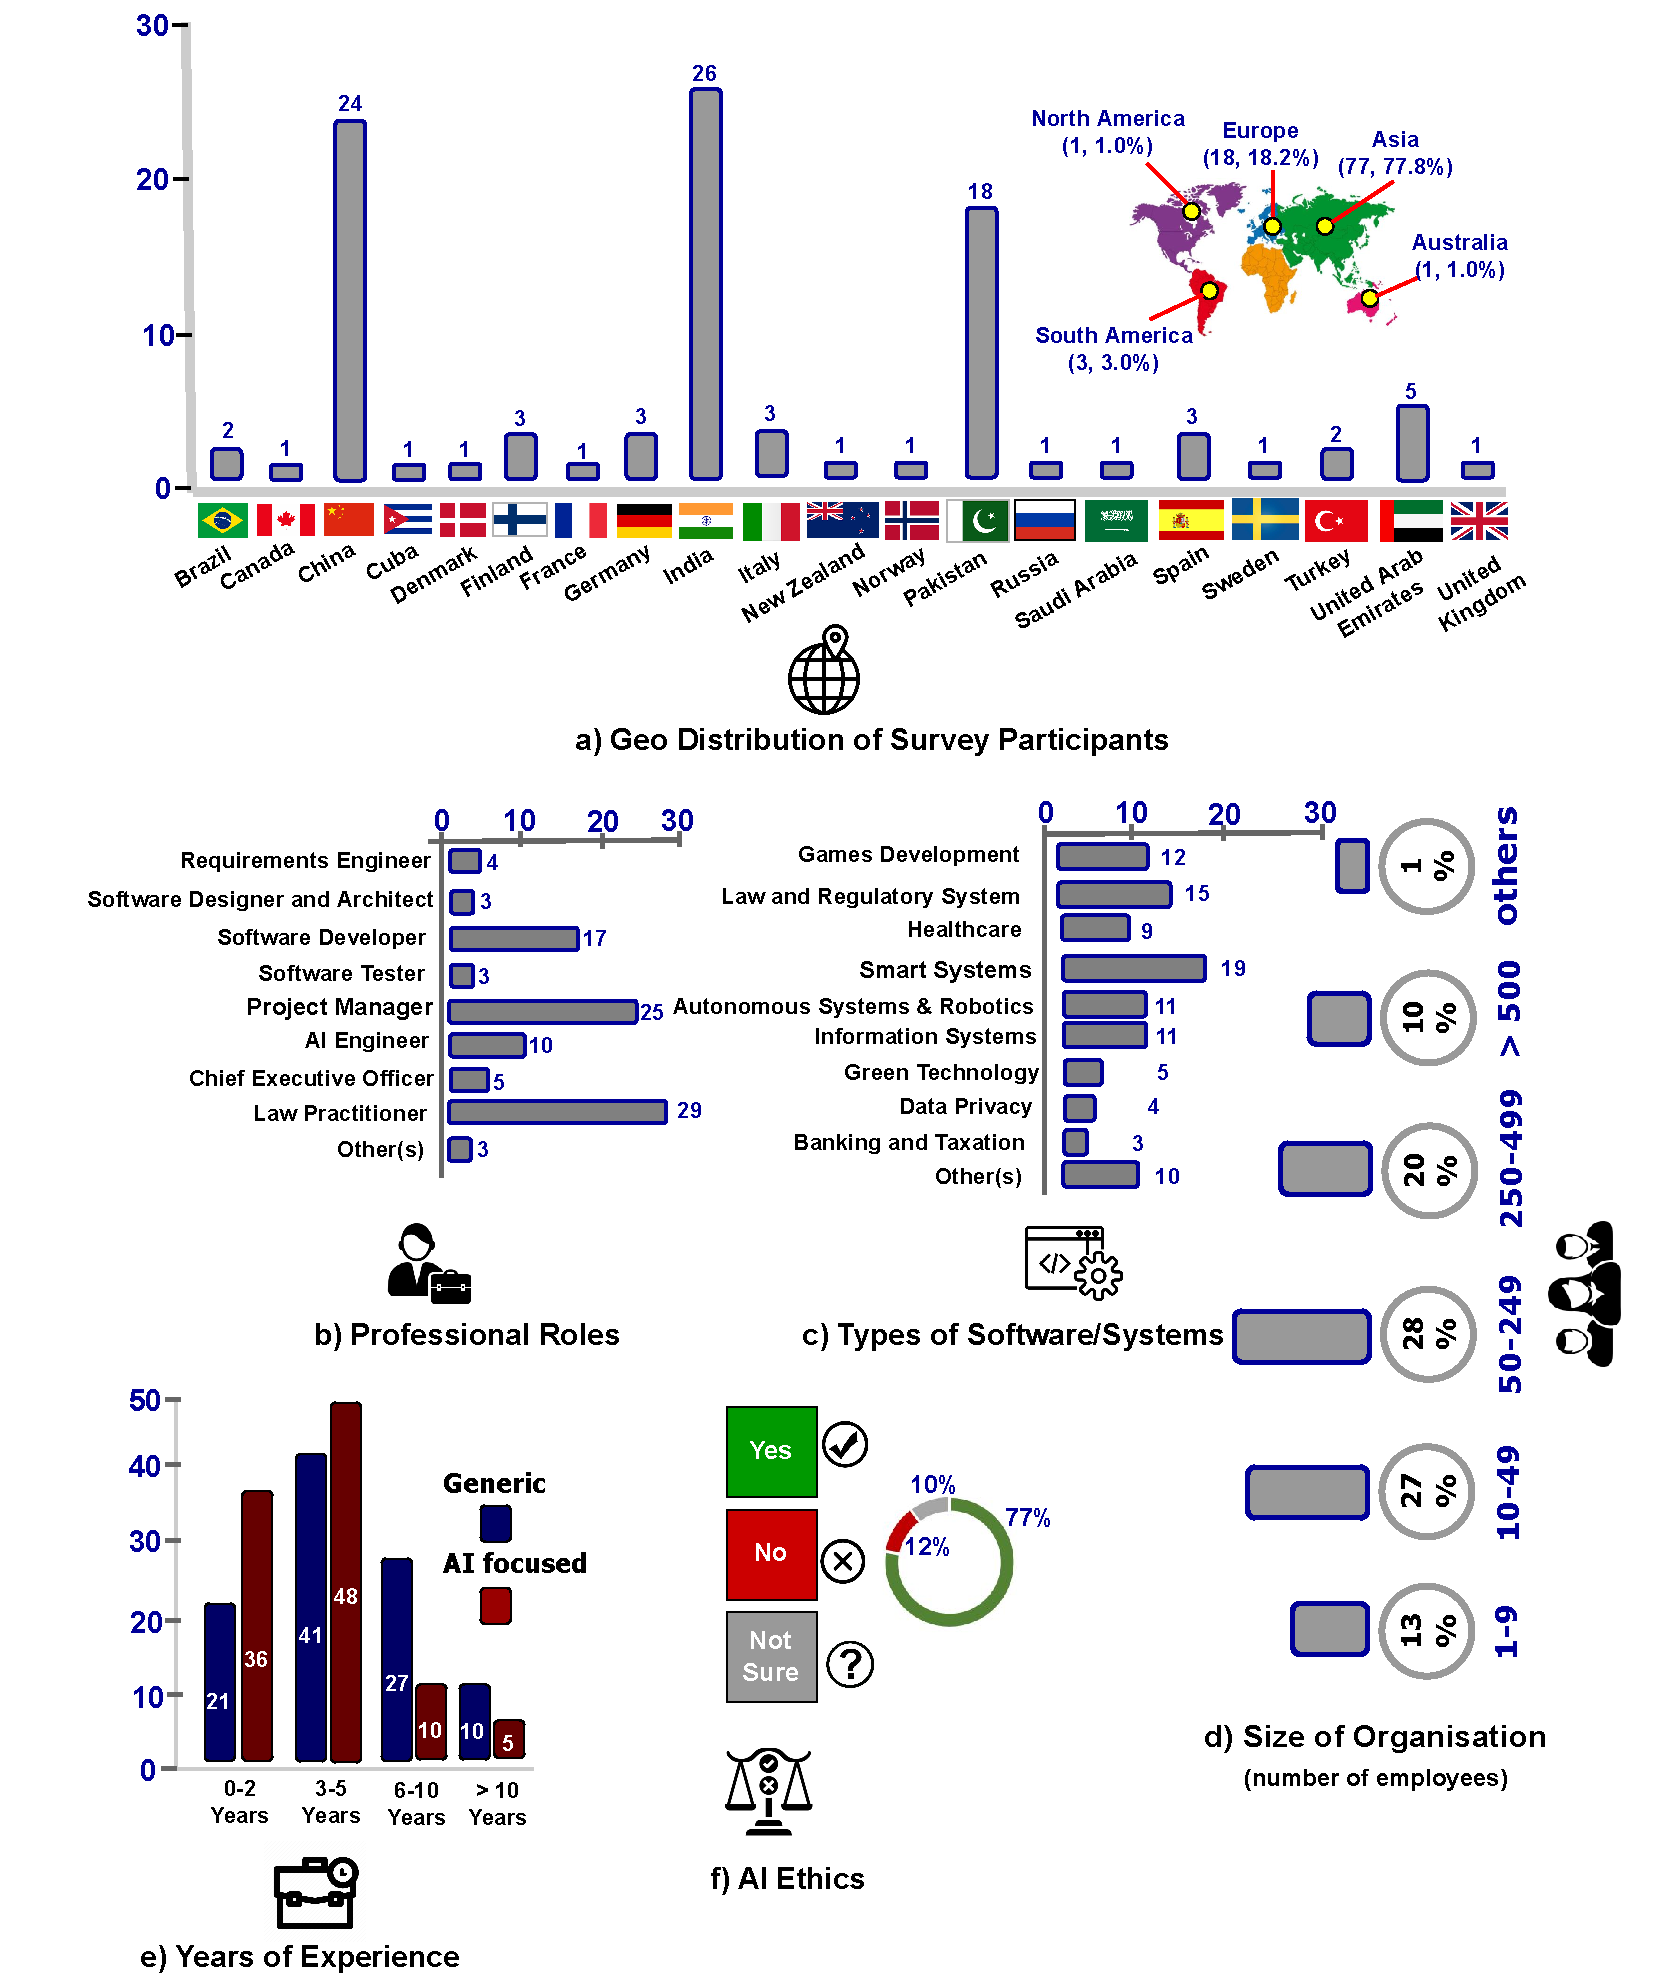
\includegraphics[scale=0.3]{Figures/Demographics.pdf} 
\centerline{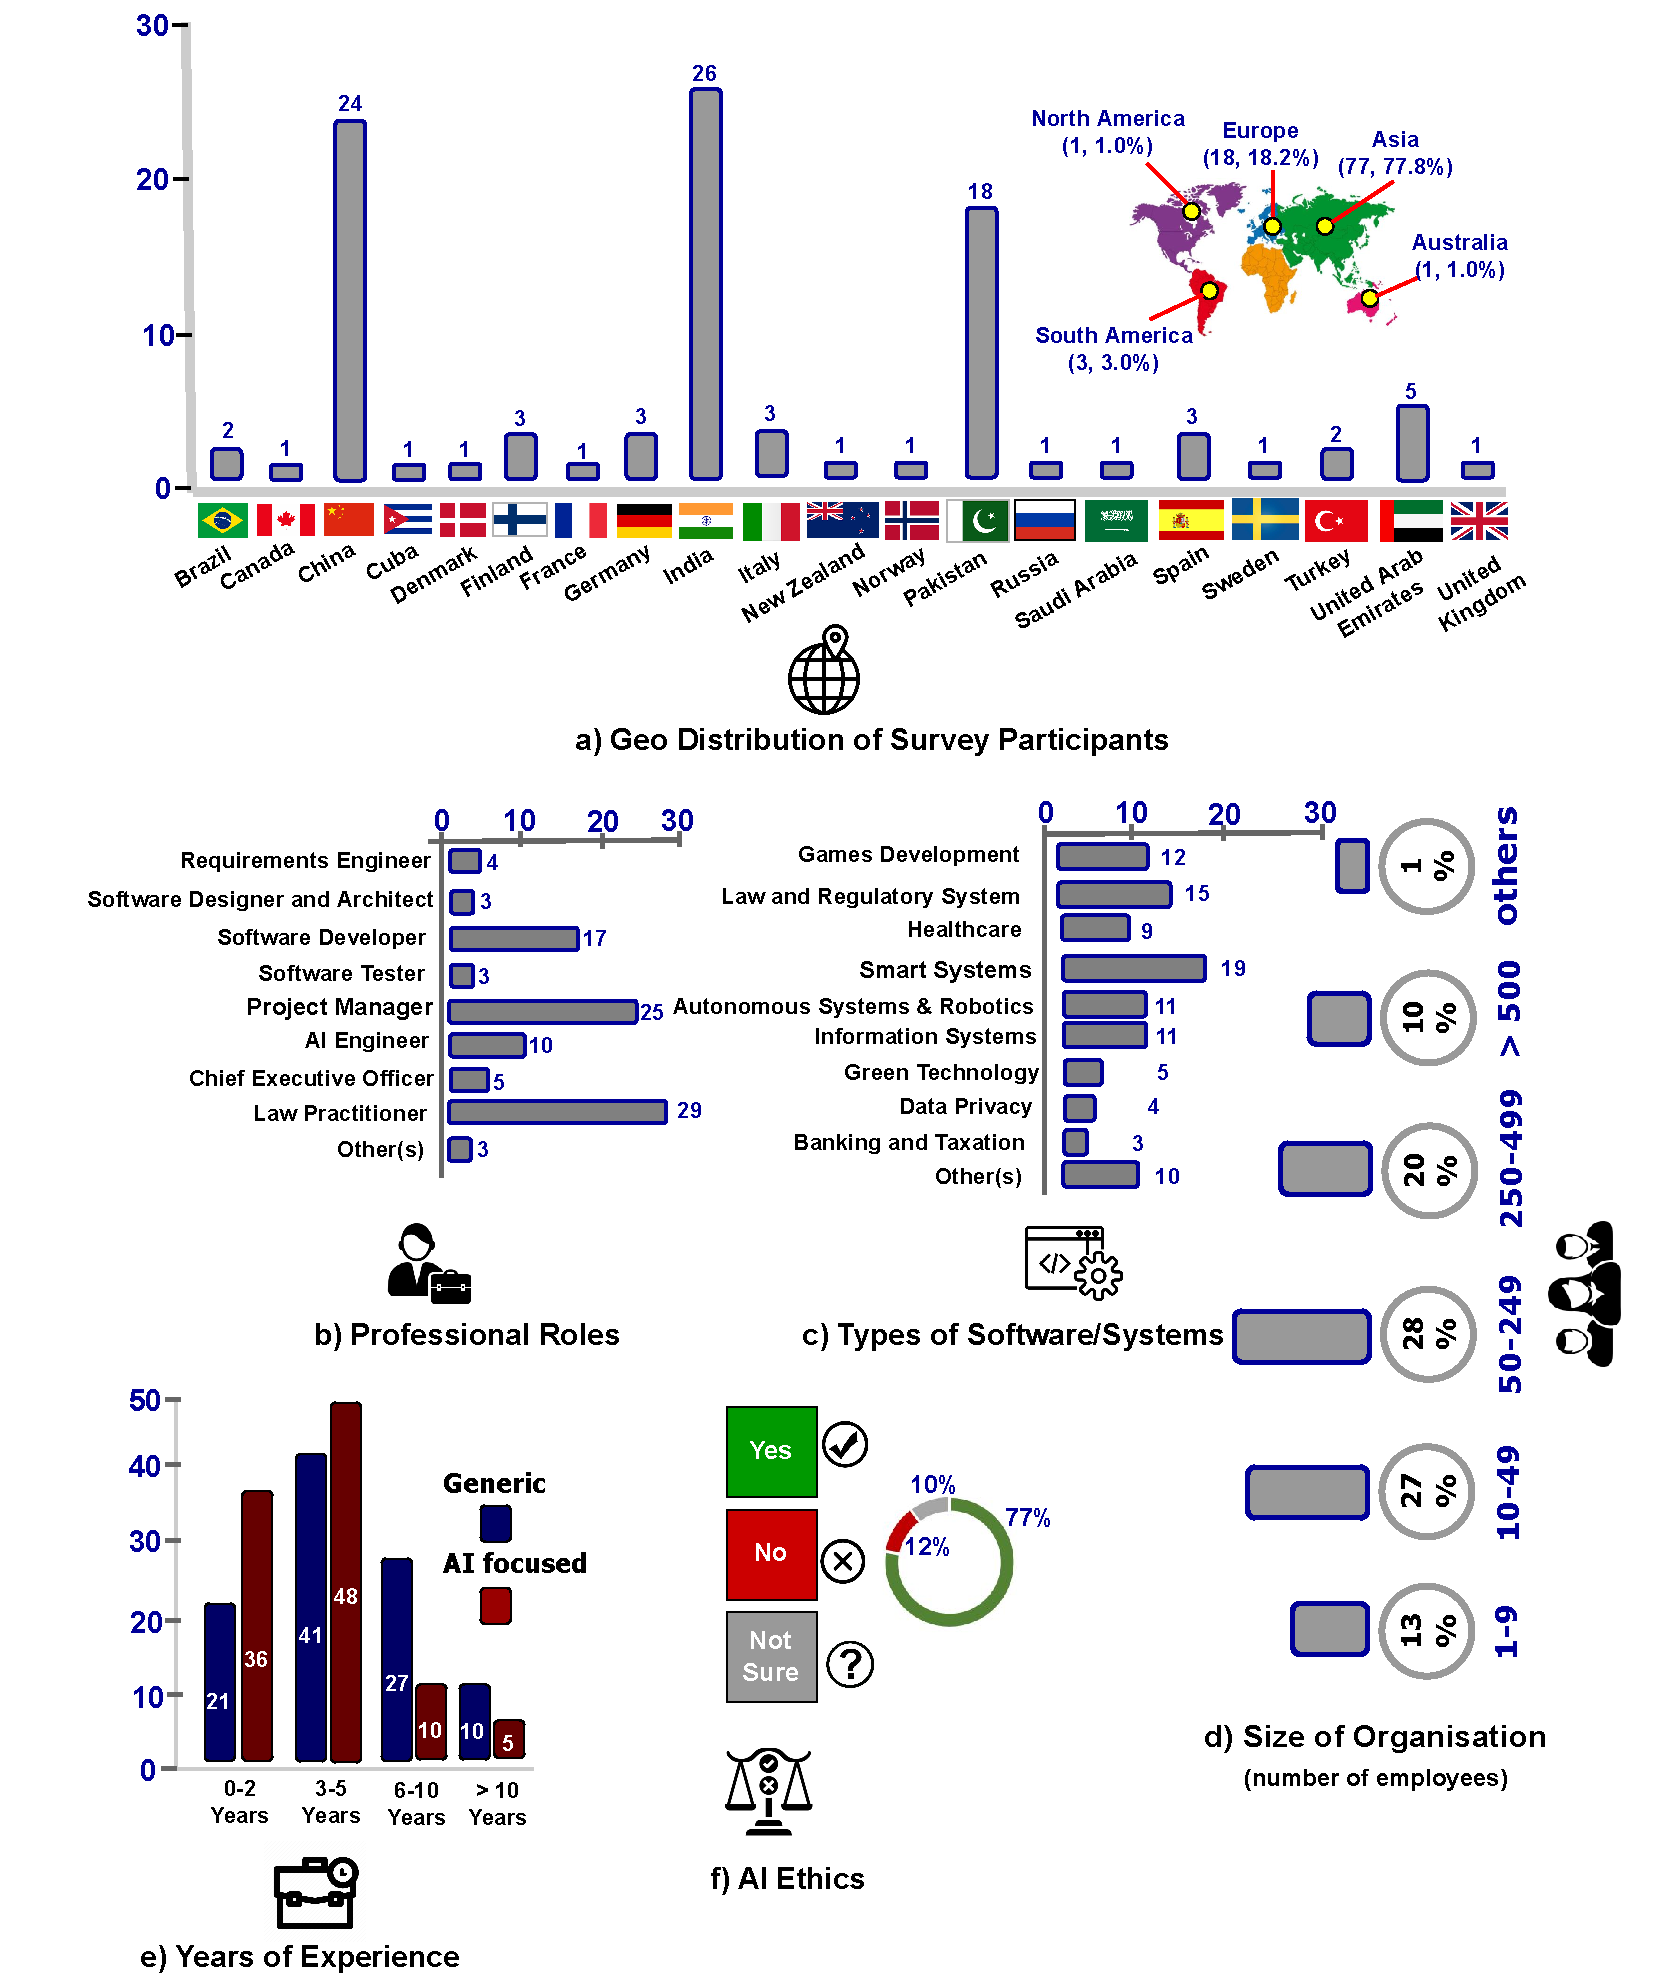
\includegraphics[width=0.8\textwidth]{Figures/Demographics.pdf}}
\caption{Demographic details of survey participants}
	\label{Fig:Demographics}
\end{figure*}

\subsection{AI ethics principles and challenges (RQ1)} \label{sec:AI ethics principles and challenges (RQ1)}

The survey responses are classified as average agree, neutral and average disagree (see Figure \ref{Fig:SurveyFindings}(a-b)). We observed that (approx. 65\%) of the respondents positively confirmed the AI ethics principles and challenges identified in the SLR study \cite{AR13}. 

\begin{figure*}
\centering
%\setlength{\fboxrule}{1pt}
% 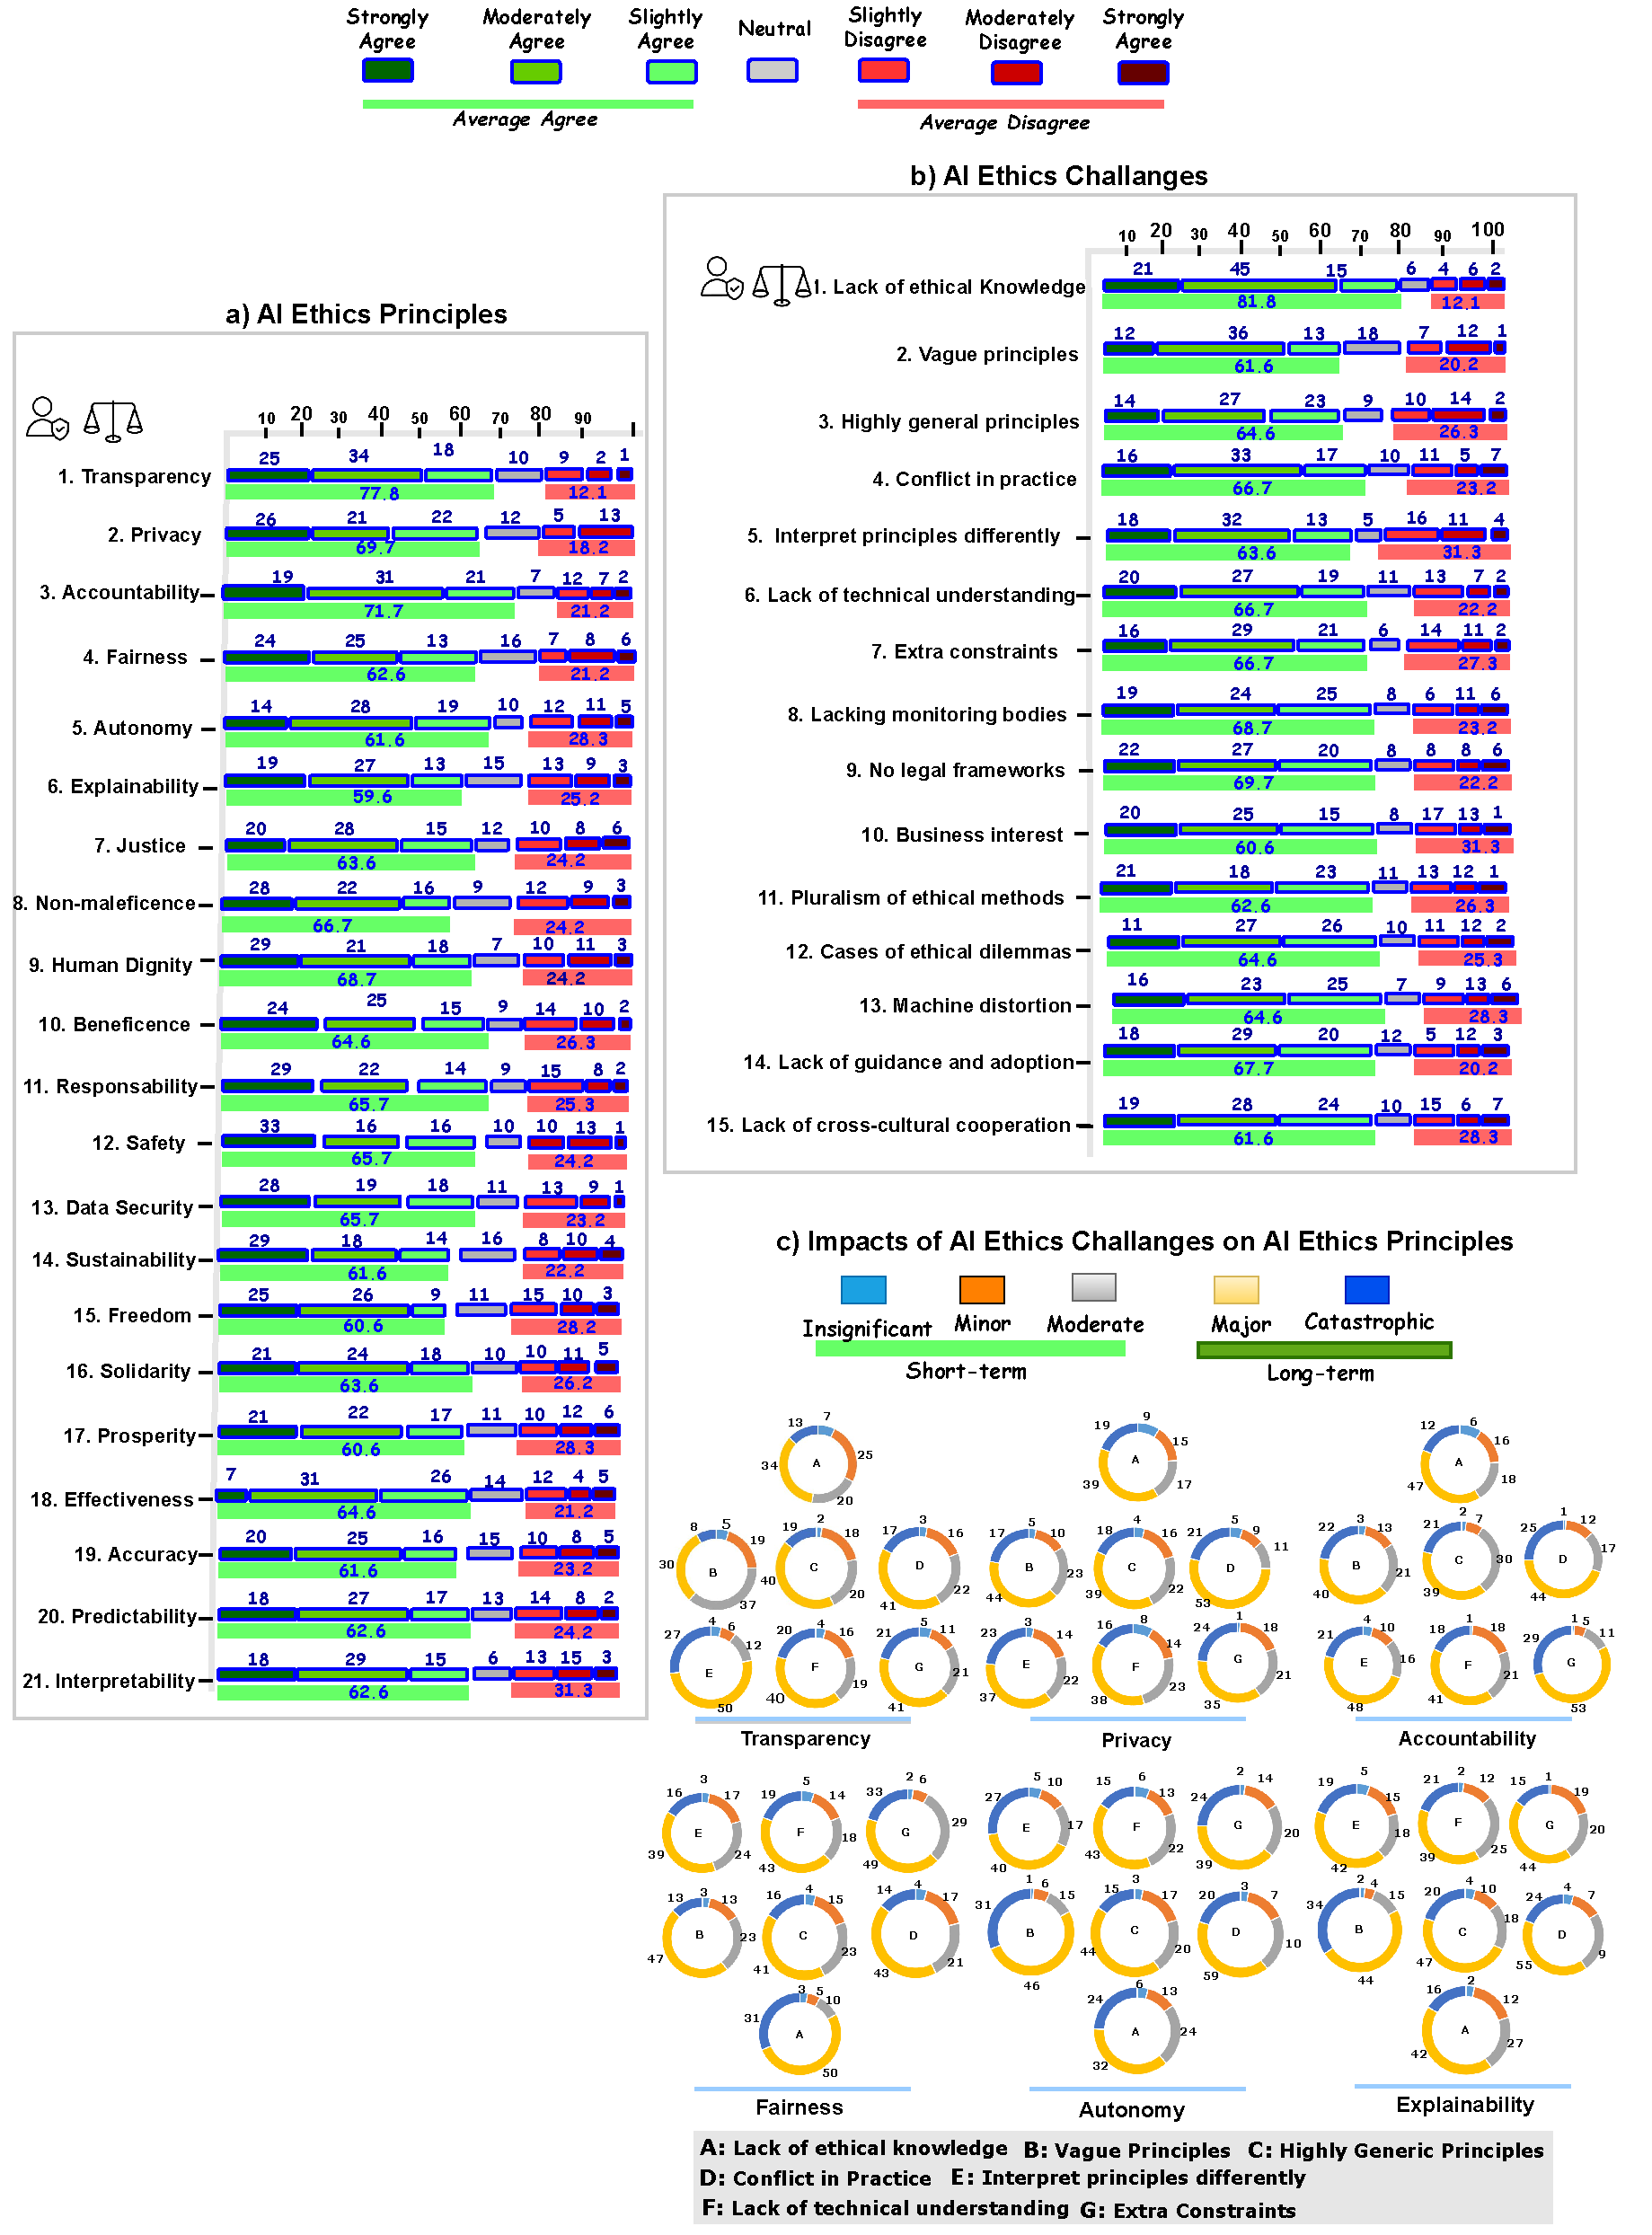
\includegraphics[scale=0.41]{Figures/SurveyFindings.pdf} 
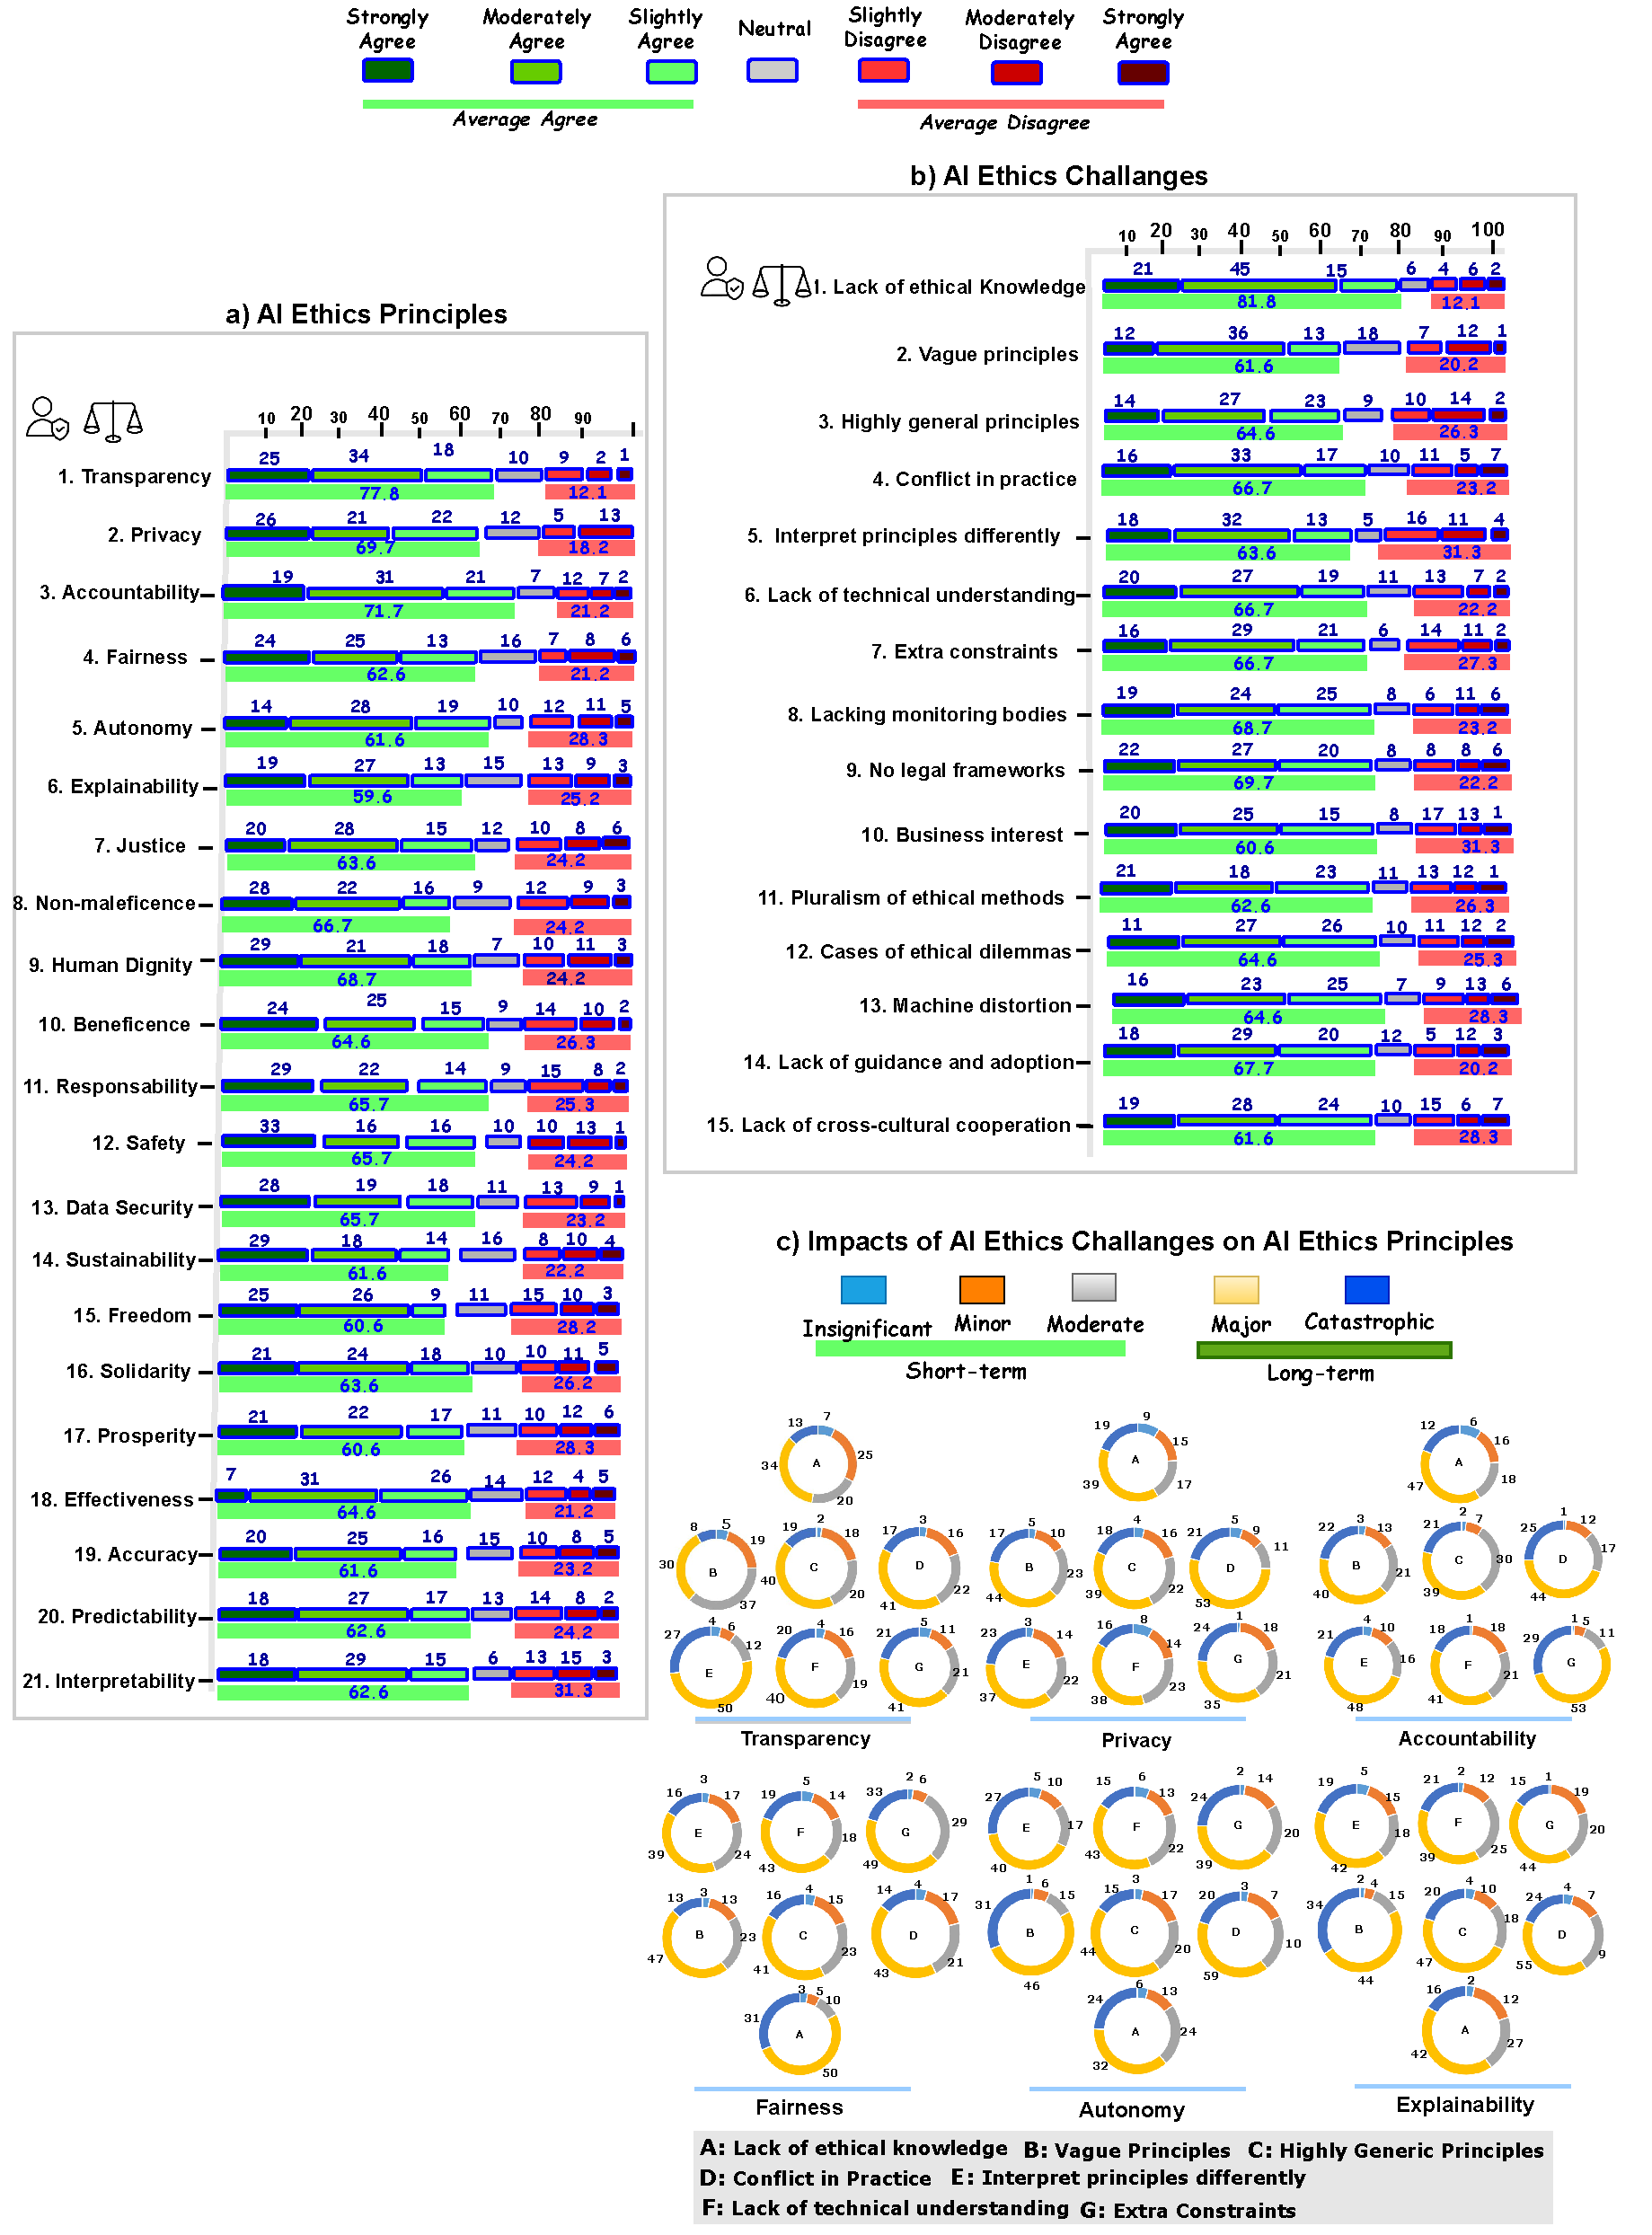
\includegraphics[width=0.95\textwidth]{Figures/SurveyFindings.pdf}
 	\caption{Survey participants perceptions on AI ethics principles and challenges}
	\label{Fig:SurveyFindings}
\end{figure*}

\subsubsection{AI ethics principles}
The results illustrate that the majority of the survey participants positively agreed (approx. 64\%) to consider the identified list of AI ethics principles (see Figure \ref{Fig:SurveyFindings}(a)). For instance, one survey participant mentioned that: 

\faComment{} “\textit{The listed AI ethics principles are comprehensive and extensive to cover various aspects of ethics in AI.}” 

We noticed that 77.8\% of survey respondents thought \textit{transparency} as the most significant AI ethics principle. This is an interesting observation as \textit{transparency} is equally confirmed as one of the core seven essential requirements by AI HLEG \cite{AR2} for realizing the ‘trustworthy AI’. \textit{Transparency} provides detailed explanations of logical AI models and decision-making structures understandable to the system stakeholders. Moreover, it deals with the public perceptions and understanding of how AI systems work. Broadly, it is a societal and normative ideal of “openness”.

The second most significant principle to the survey participants was \textit{accountability} (71.7\%). It refers to the expectations or requirements that the organizations or individuals need to ensure throughout the lifecycle of an AI system. They should be accountable according to their roles and applicable regulatory frameworks for the system design, development, deployment, and operation by providing documentation on the decision-making process or conducting regular auditing with proper justification. \textit{Privacy} is the third most frequently occurred principle, supported by 69.7\% of the survey participants. It refers to preventing harm, a fundamental right specifically affected by the decision-making system. \textit{Privacy} compels data governance throughout the system lifecycle, covering data quality, integrity, application domain, access protocols, and capability to process the data in a way that safeguards privacy. It must be ensured that the data collected and manipulated by the AI system shall not be used unlawfully or unfairly discriminate against human beings. For example, one of the respondents mentioned that 

\faComment{} “\textit{The privacy of hosted data used in AI applications and the risk of data breaches must be considered.}” 

In general, the survey findings of AI ethics principles are confirmatory to the widely adopted accountability, responsibility, and transparency (ART) framework \cite{AR15} and the findings of an industrial empirical study conducted by Ville et al. \cite{AR10}. Both studies \cite{AR10} \cite{AR15} jointly considered \textit{transparency} and \textit{accountability} as the core AI ethics principles, which is consistent with the findings in this survey. On contrary, we noticed that \textit{privacy} has been ignored in both mentioned studies \cite{AR10} \cite{AR15}, but is placed as the third most significant principle in this survey. The reason might be that, as more and more AI systems have been placed online, the significance of \textit{privacy} and data protection is increasingly recognized \cite{bansal2022internet}. Presently, various countries embarked on legislation to ensure the protection of data and \textit{privacy}.

\subsubsection{AI ethics challenges}

Further, the results reveal that the majority of the survey respondents (approx. 66\%) confirmed the identified challenging factors \cite{AR13} (see Figure \ref{Fig:SurveyFindings}(b)). \textit{Lack of ethical knowledge} is considered as the most frequently cited challenge by (81.8\%) of the survey participants. It exhibits that knowledge of ethical aspects across AI systems is largely ignored in industrial settings. There is a significant gap between research and practice in AI ethics. Extant guidelines and policies devised by researchers and regulatory bodies discussed different ethical goals for AI systems. However, these goals have not been widely adopted in the industrial domain because of limited knowledge of scaling them in practice. The findings are in agreement with the results of industrial study conducted by Ville et al. \cite{AR10}, concluding that ethical aspects of AI systems are not exclusively considered, and it mainly happened because of a lack of knowledge, awareness, and personal commitment. We noticed that \textit{no legal frameworks} (69.7\%) is ranked as the second most common challenge for considering ethics in the AI domain. The proliferation of AI technologies in high-risk areas starts mounting the pressure of designing ethical and legal standards and frameworks to govern them \cite{cath2018governing}. It highlights the nuances of the debate on AI law and lays the groundwork for a more inclusive AI governance framework \cite{schiff2020s}. The framework shall focus on most pertinent ethical issues raised by the AI systems, the use of AI across industry and government organisations, and economic displacement (i.e. the ethical reply to the loss of jobs as a result of AI-based automation). The third most common challenging factor is \textit{lacking monitoring bodies}, and it was highlighted by (68.7\%) of the survey participants. \textit{Lacking monitoring bodies} refers to the lack of regulatory oversight to assess ethics in AI systems \cite{AR13}. It raises the issue of public bodies’ empowerment to monitor, and audit the enforcement of ethical concerns in AI technologies by the domain (e.g., health, transport, education). One survey respondent mentioned that 

\faComment{} “\textit{I believe it shall be mandatory for the industry to get standard approval from monitoring bodies to consider ethics in the development process of AI systems.}” 

Monitoring bodies extensively promote and observe the ethical values in society and evaluate technology development associated with ethical aspects of AI \cite{AR2}. They would be tasked to advocate and define responsibilities and develop rules, regulations, and practices in a situation where the system takes a decision autonomously. The monitoring group should ensure “ethics by, in and for design” as mentioned in AI HLEG \cite{AR2} guidelines. 

Additionally, the survey participants elaborated on new challenging factors. For instance, one of the participants mentioned that 

\faComment{}  “\textit{Implicit biases in AI algorithms such as data discrimination and cognitive biases could impact system transparency.}” 

Similarly, the other respondent reported that 

\faComment{} “\textit{Biases in the AI system’s design might bring distress to a group of people or individuals.}” 

Moreover, a survey respondent explicitly considered the \textit{lack of tools for ethical transparency} and \textit{AI biases} as significant challenges to AI ethics. We noticed that \textit{AI biases} is reported as the most common additional challenge. It will be interesting to further explore (i) the type of biases that might be embedded with the AI algorithms, (ii) the causes of these biases, and (iii) corresponding countermeasures to minimize the negative impact on AI ethics.

\subsection{Severity impacts of identified challenges (RQ2)} \label{sec:Severity impacts of identified challenges (RQ2)}

We selected the most frequently reported seven challenging factors and six principles discussed in our SLR study \cite{AR13}. The aim is to investigate the severity impact of the seven challenges \textit{(i.e., lack of ethical knowledge, vague principles, highly general principles, conflict in practice, interpret principles differently, lack of technical understanding, and extra constraints)} across the six AI ethics principles \textit{(i.e. transparency, privacy, accountability, fairness, autonomy, and explainability)}. The survey participants were asked to rate the severity impact using the Likert scale: short-term (insignificant, minor, moderate) and long-term (major, and catastrophic)  (see Figure \ref{Fig:SurveyFindings}(c)). The results revealed that most challenges have long-term impacts on the principles (major, and catastrophic). 

For the \textit{transparency} principle, we noticed that the challenging factor \textit{interpret principles differently} has significant long-term impacts, and 77\% (i.e., 50\% major, and 27\% catastrophic) of the survey participants agreed to it. The interpretation of ethical concepts can change for a group of people and individuals. For instance, the practitioners might perceive \textit{transparency} differently (more focused on technical aspects) than law and policymakers, who have broad social concerns. Furthermore, \textit{lack of ethical knowledge} has a short-term impact on the \textit{transparency} principle, and it is evident from the survey findings supported by 52\% (7\% insignificant, 25\% minor, and 20\% moderate) responses. Lack of knowledge could be instantly covered by attaining knowledge, understanding, and awareness of transparency concepts. 

\textit{Conflict in practice} is deemed the most significant challenge to the \textit{privacy} principle. Hence, 74\% (i.e., 53\% major, and 21\% catastrophic) survey respondents considered it a long-term severe challenge. Various groups, organizations, and individuals might have opinion conflicts associated with \textit{privacy} in AI ethics \cite{stahl2018ethics}. It is critical to interpret and understand privacy conflicts in practice. We noticed that (82\%) of survey participants considered the challenging factor \textit{extra constraints} as the most severe (long-term) challenge for both \textit{accountability} and \textit{fairness} principles. Situational constraints, including organizational politics, lack of information, and management interruption, could possibly interfere with the accountability and fairness measures \cite{krijger2021enter}. It could negatively impact the employee’s motivation and interest to explicitly consider ethical aspects across the AI activities. Interestingly, (79\%) of the survey respondents considered \textit{conflict in practice} as the most common (long-term) challenge for \textit{autonomy} and \textit{explainability} principles.

Overall, we could interpret that \textit{conflict in practice}  is the most severe challenge, and its average occurrence is $>$60\% for all the principles. It gives a general understanding to propose specific solutions that focus on tackling the opinion conflict regarding the real-world implication of AI ethics principles. The results further reveal \textit{lack of ethical knowledge} has an average (28\%) short-term impact across selected AI ethics principles. The lack of knowledge gap could be covered by conducting training sessions, workshops, certification, and encouraging social awareness of AI ethics \cite{AR13}. Knowledge increases the possibility of AI ethics success and acceptance in the best practice of the domain. 

\subsection{Statistical inferences (RQ3)} \label{sec:Statistical inferences (RQ3)}

We performed non-parametric statistical analysis \cite{myers2004spearman}\cite{de2016comparing} to evaluate the significant differences  and similarities between the opinion of lawmakers and software practitioners. The same non-parametric statistical analysis are previously performed in different other similar nature of studies  \cite{akbar2022srcmimm}\cite{khan2020systematic}\cite{khan2017systematic}. The frequency-based ranking of both datasets is identified for AI ethics principles (see Table \ref{tab:Rank-Principles}) and challenges (see Table  \ref{tab:AI ethics challenges ranks}) to set common measures for non-parametric Spearman's Rank-order correlation coefficient. It gives the linear  dependence between a set of variables, ranging from (rs (co-relation coefficient) = +1 to -1), where +1 indicates a total linear dependency \cite{myers2004spearman}\cite{de2016comparing}.

\subsubsection{Significant differences for AI ethics principles}

The Spearman's Rank-order correlation test was applied to statistically evaluate the significant differences between the practitioners and lawmakers perceptions on AI ethics principles. We obtained the Spearman's Rank-order correlation coefficient value (rs$=$0.819), which is statistically significant (p$=$0.000) (see Table \ref{tab:correlation_Principles}). The value (rs$=$0.819) and the scatter plot given in Figure \ref{Fig:Scatter-Ranks-Principles} show the strong correlation between the ranks of both datasets (lawmakers and software practitioners). The identified principles are widely discussed across multiple AI ethics guidelines, and it might be the reason why both practitioners and lawmakers equally agreed with the significance and implications of these principles. For example, \textit{transparency} is a common AI ethics principle, and practitioners and lawmakers ranked it in the first position. However, we also noticed significant differences (p$=$0.000) between both types of the population. For instance, lawmakers ranked \textit{fairness} at position five as the most important principle; however, the software practitioners placed it at position seven. It shows that fairness across AI activities is relatively important based on lawmakers' perceptions. It is because \textit{fairness} is a non-technical and more socially used term. Laws like EU GDPR impose concrete requirements on AI development organizations to safeguard fairness in AI system design, deployment, and data processing \cite{GDPR}. The low-ranked placement of \textit{fairness} by the practitioners might be because of limited knowledge and understanding of interpreting fairness technically, e.g., fairness in AI by design.

\begin{table*}[htbp] 
\centering
\caption{AI ethics principles ranks}
\label{tab:Rank-Principles}
% \resizebox{0.8\textwidth}{!}{%
\begin{tabular}{|l|c|c|c|c|}
\hline
\multicolumn{1}{|c|}{\textbf{Principles}} & \multicolumn{1}{c|}{\textbf{\begin{tabular}[c]{@{}c@{}}Lawmaker\\ (n=29)\end{tabular}}} & \multicolumn{1}{c|}{\textbf{\begin{tabular}[c]{@{}c@{}}Rank by\\ Lawmakers\end{tabular}}} & \multicolumn{1}{c|}{\textbf{\begin{tabular}[c]{@{}c@{}}Practitioners\\ (n=52)\end{tabular}}} & \multicolumn{1}{c|}{\textbf{\begin{tabular}[c]{@{}c@{}}Rank by\\ Practitioners\end{tabular}}} \\ \hline
Transparency & 25 & 1 & 52 & 1 \\ \hline
Privacy & 23 & 3 & 43 & 4 \\ \hline
Accountability & 24 & 2 & 44 & 3 \\ \hline
Fairness & 21 & 5 & 39 & 7 \\ \hline
Autonomy & 20 & 6 & 39 & 7 \\ \hline
Explainability & 19 & 7 & 38 & 8 \\ \hline
Justice & 20 & 6 & 41 & 5 \\ \hline
Non-maleficence & 23 & 3 & 41 & 5 \\ \hline
Human dignity & 24 & 2 & 44 & 3 \\ \hline
Beneficence & 22 & 4 & 44 & 3 \\ \hline
Responsibility & 22 & 4 & 43 & 4 \\ \hline
Safety & 23 & 3 & 44 & 3 \\ \hline
Data Security & 22 & 4 & 41 & 5 \\ \hline
Sustainability & 24 & 2 & 45 & 2 \\ \hline
Freedom & 21 & 5 & 39 & 7 \\ \hline
Solidarity & 21 & 5 & 41 & 5 \\ \hline
Prosperity & 20 & 6 & 40 & 6 \\ \hline
Effectiveness & 20 & 6 & 43 & 4 \\ \hline
Accuracy & 21 & 5 & 40 & 6 \\ \hline
Predictability & 23 & 3 & 43 & 4 \\ \hline
Interpretability & 21 & 5 & 40 & 6 \\ \hline
\end{tabular}%
% }
\end{table*}

% Please add the following required packages to your document preamble:
% \usepackage{multirow}
% Please add the following required packages to your document preamble:
% \usepackage{multirow}
\begin{table*}[htbp]
\centering
\caption{Practitioners and lawmakers perceptions co-relation for AI ethics principles}
\label{tab:correlation_Principles}
% \resizebox{0.8\textwidth}{!}{%
\begin{tabular}{|lllrr|}
\hline
\multicolumn{3}{|l|}{} & \multicolumn{1}{c|}{\begin{tabular}[c]{@{}c@{}}Lwawmakers\_\\ Ranking\_pra\end{tabular}} & \multicolumn{1}{c|}{\begin{tabular}[c]{@{}c@{}}Practitioners\_\\ Ranking\_pra\end{tabular}} \\ \hline
\multicolumn{1}{|l|}{\multirow{6}{*}{Spearman's rho}} & \multicolumn{1}{c|}{\multirow{3}{*}{\begin{tabular}[c]{@{}c@{}}Lwawmakers\_\\ Ranking\_pra\end{tabular}}} & \multicolumn{1}{l|}{Correlation Coefficient} & \multicolumn{1}{r|}{1.000} & 0.819** \\ \cline{3-5} 
\multicolumn{1}{|l|}{} & \multicolumn{1}{c|}{} & \multicolumn{1}{l|}{Sig. (2-tailed)} & \multicolumn{1}{r|}{.} & 0.000 \\ \cline{3-5} 
\multicolumn{1}{|l|}{} & \multicolumn{1}{c|}{} & \multicolumn{1}{l|}{N} & \multicolumn{1}{r|}{21} & 21 \\ \cline{2-5} 
\multicolumn{1}{|l|}{} & \multicolumn{1}{l|}{\multirow{3}{*}{\begin{tabular}[c]{@{}l@{}}Practitioners\_\\ Ranking\_pra\end{tabular}}} & \multicolumn{1}{l|}{Correlation Coefficient} & \multicolumn{1}{r|}{0.819**} & 1.000 \\ \cline{3-5} 
\multicolumn{1}{|l|}{} & \multicolumn{1}{l|}{} & \multicolumn{1}{l|}{Sig. (2-tailed)} & \multicolumn{1}{r|}{0.000} & . \\ \cline{3-5} 
\multicolumn{1}{|l|}{} & \multicolumn{1}{l|}{} & \multicolumn{1}{l|}{N} & \multicolumn{1}{r|}{21} & 21 \\ \hline
\multicolumn{5}{|l|}{**. Correlation is significant at the 0.01 level (2-tailed).} \\ \hline
\end{tabular}%
% }
\end{table*}

\begin{figure}[]
\centering
%\setlength{\fboxrule}{1pt}
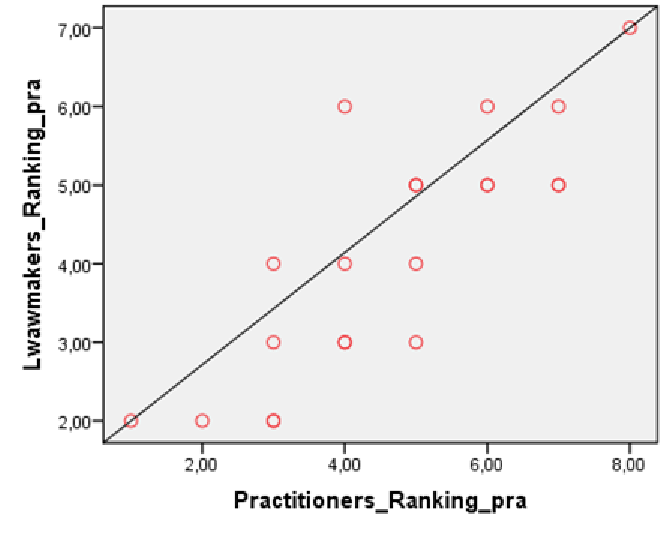
\includegraphics[width=0.4\textwidth]{Figures/Pract-ranking.drawio.pdf} 
%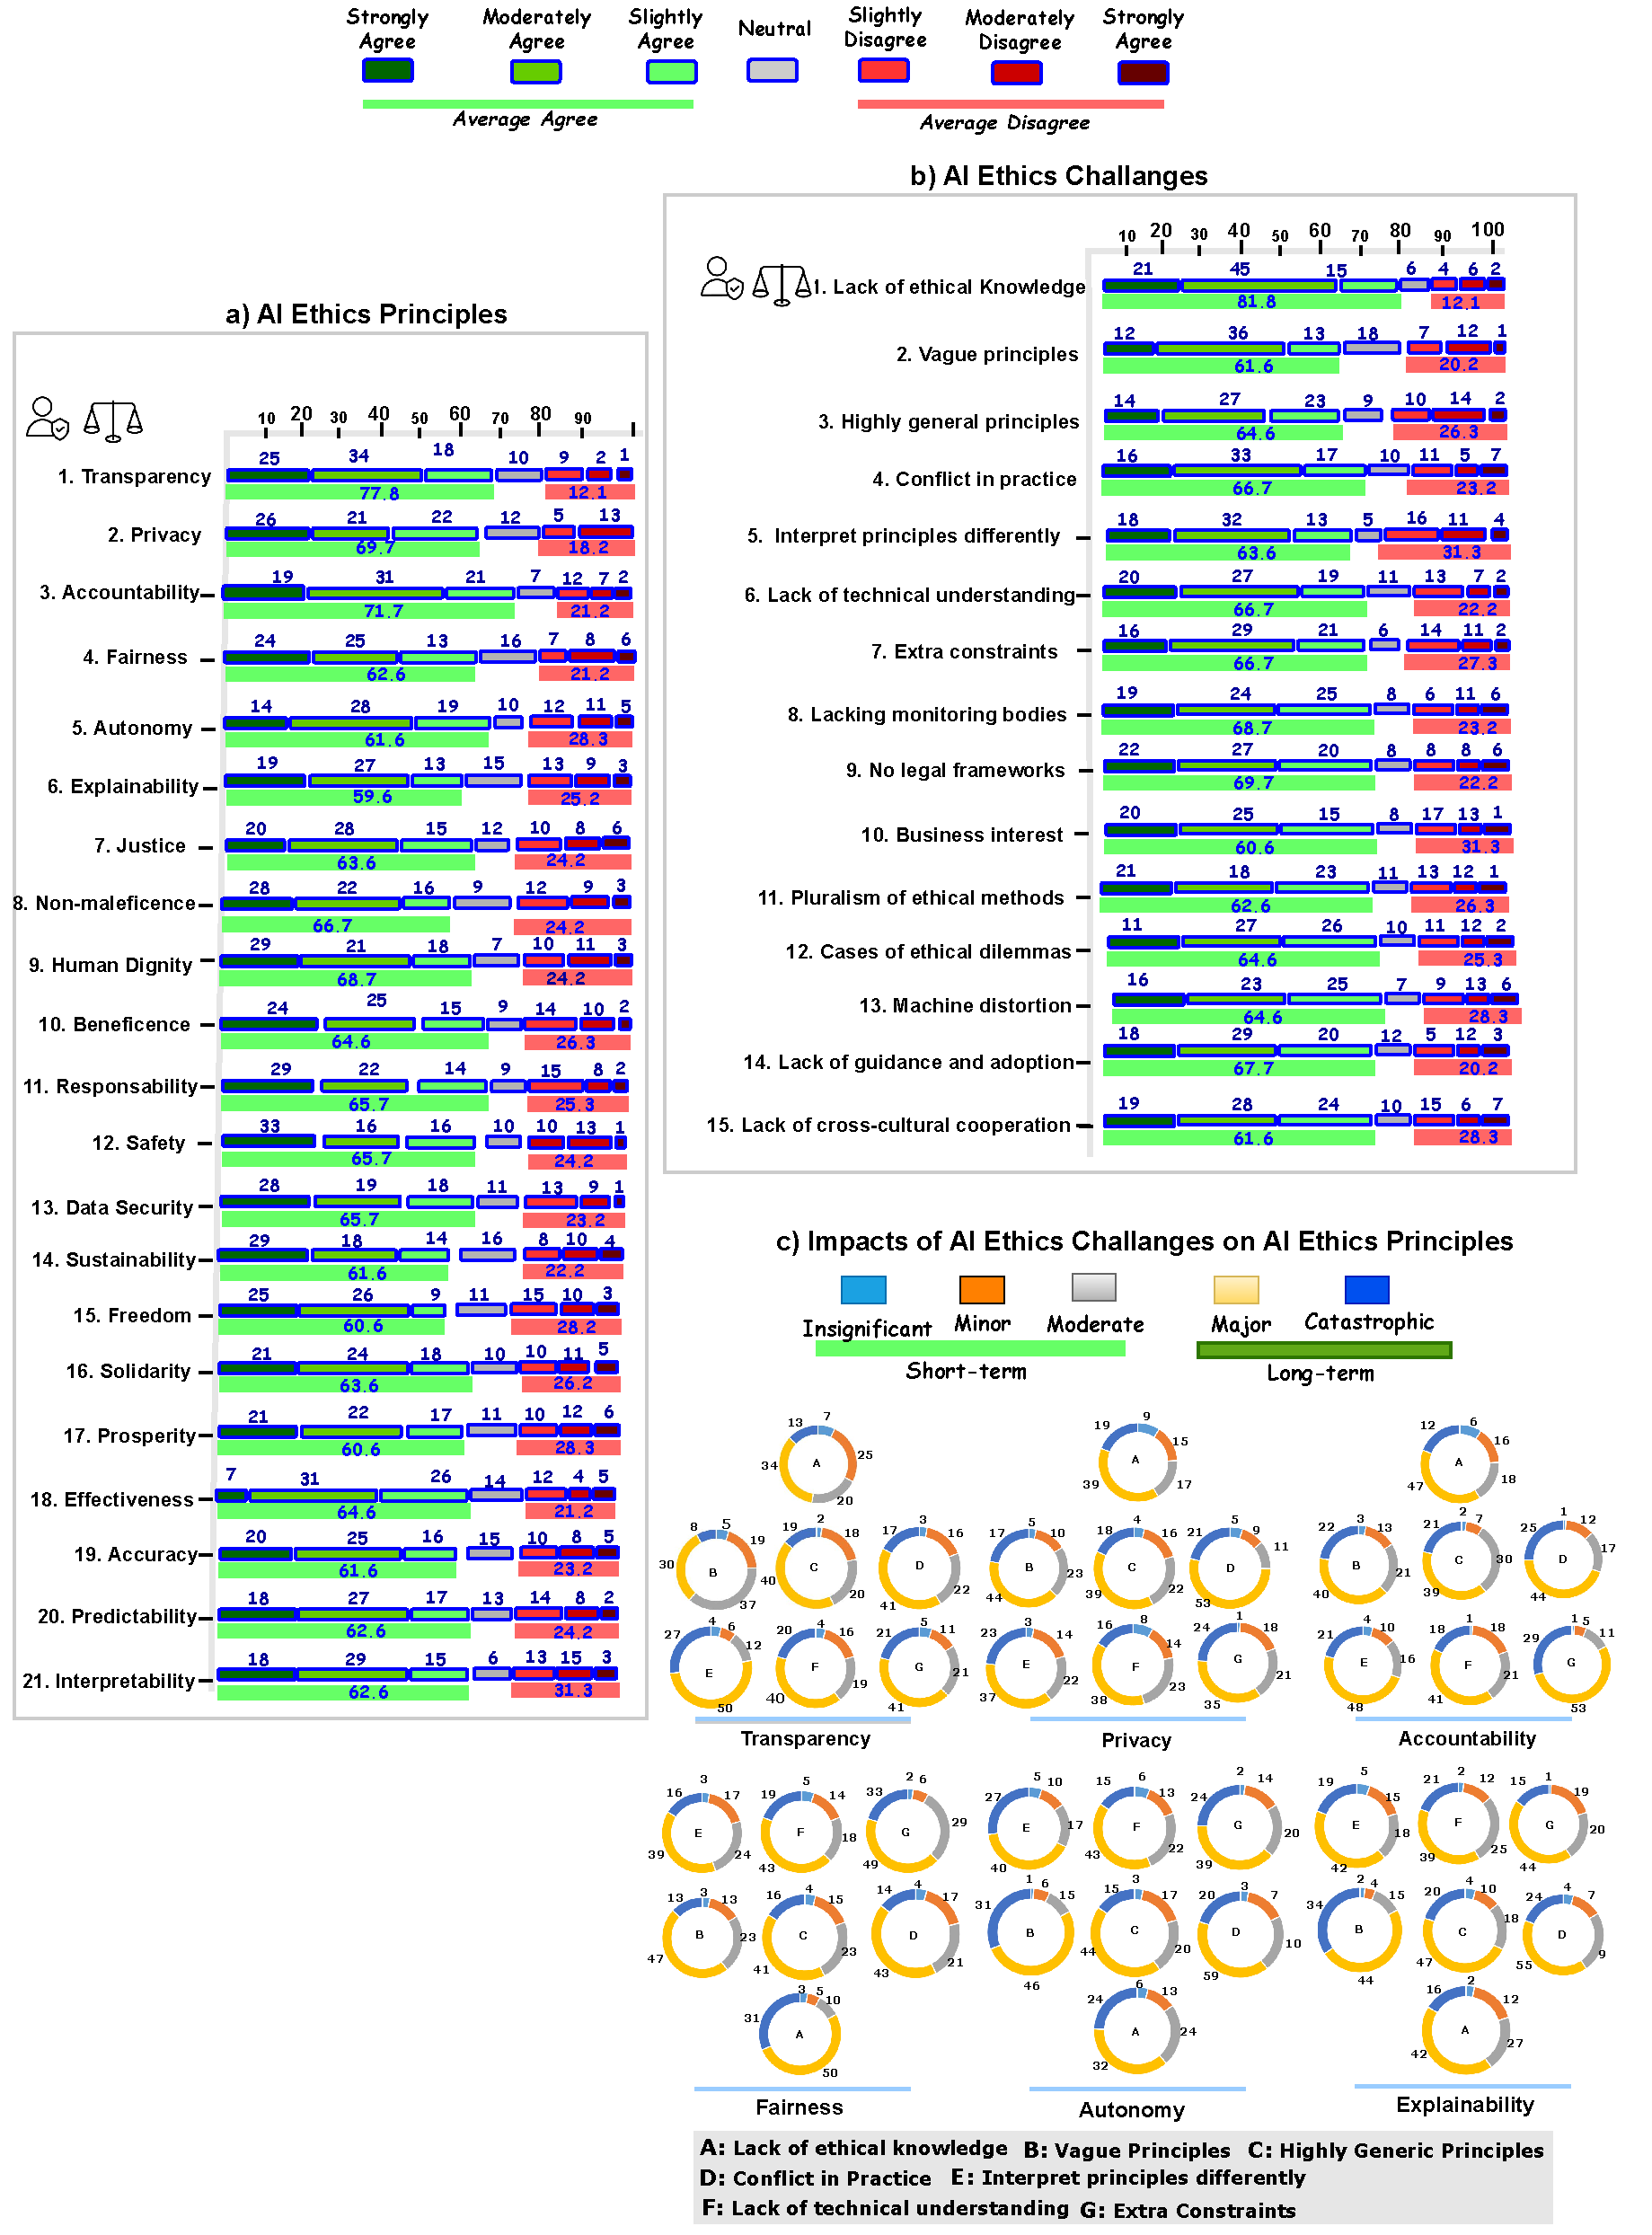
\includegraphics[width=\textwidth]{Figures/SurveyFindings.pdf}
 	\caption{Scatter plot of ranks for AI ethics principles}
	\label{Fig:Scatter-Ranks-Principles}
\end{figure}

In addition to Spearman's Rank order co-relation, we also applied the independent t-test to compare the mean differences of the ranks obtained from both types of population (see Table \ref{tab:ttest_principples} and Table \ref{tab:groupstatistics_principles}). Since Levene's Test is slightly significant (i.e., p$=$0.051$>$0.05), therefore, we assume that the variances are approximately equal. Based on this assumption, the results of t-test (i.e., t $=$ 0.942, p $=$ 0.661 $>$ 0.05) show that there is no high-level significant differences between both variables. The results show that the degree of agreement between lawmakers and practitioners concerning AI ethics principles is positive. It means that both populations (lawmakers and software practitioners) equally consider the importance of AI ethics principles. The group statistics for both variables are given in Table \ref{tab:groupstatistics_principles}.

\begin{table*}[]
\centering
\caption{Independent samples t-test of AI ethics principles}
\label{tab:ttest_principples}
% \resizebox{0.8\textwidth}{!}{%
\begin{tabular}{|ll|cc|ccccccr|}
\hline
\multicolumn{2}{|l|}{\multirow{3}{*}{}} & \multicolumn{2}{c|}{\begin{tabular}[c]{@{}c@{}}Levene's Test \\ for Equality \\ of Variances\end{tabular}} & \multicolumn{7}{c|}{t-test for Equality of Means} \\ \cline{3-11} 
\multicolumn{2}{|l|}{} & \multicolumn{1}{c|}{\multirow{2}{*}{F}} & \multirow{2}{*}{Sig.} & \multicolumn{1}{c|}{\multirow{2}{*}{t}} & \multicolumn{1}{c|}{\multirow{2}{*}{df}} & \multicolumn{1}{c|}{\multirow{2}{*}{\begin{tabular}[c]{@{}c@{}}Sig. \\ (2-tailed)\end{tabular}}} & \multicolumn{1}{c|}{\multirow{2}{*}{\begin{tabular}[c]{@{}c@{}}Mean \\ Difference\end{tabular}}} & \multicolumn{1}{c|}{\multirow{2}{*}{\begin{tabular}[c]{@{}c@{}}Std. Error \\ Difference\end{tabular}}} & \multicolumn{2}{c|}{\begin{tabular}[c]{@{}c@{}}95\% Confidence \\ Interval of the \\ Difference\end{tabular}} \\ \cline{10-11} 
\multicolumn{2}{|l|}{} & \multicolumn{1}{c|}{} &  & \multicolumn{1}{c|}{} & \multicolumn{1}{c|}{} & \multicolumn{1}{c|}{} & \multicolumn{1}{c|}{} & \multicolumn{1}{c|}{} & \multicolumn{1}{c|}{Lower} & \multicolumn{1}{c|}{Upper} \\ \hline
\multicolumn{1}{|l|}{\multirow{2}{*}{Rank}} & \begin{tabular}[c]{@{}l@{}}Equal variances\\ assumed\end{tabular} & \multicolumn{1}{r|}{.117} & \multicolumn{1}{r|}{0.051} & \multicolumn{1}{r|}{0.942} & \multicolumn{1}{r|}{40} & \multicolumn{1}{r|}{.661} & \multicolumn{1}{r|}{-.23810} & \multicolumn{1}{r|}{.53875} & \multicolumn{1}{r|}{-1.32695} & .85076 \\ \cline{2-11} 
\multicolumn{1}{|l|}{} & \begin{tabular}[c]{@{}l@{}}Equal variances \\ not assumed\end{tabular} & \multicolumn{1}{l|}{} & \multicolumn{1}{l|}{} & \multicolumn{1}{r|}{0.942} & \multicolumn{1}{r|}{39.616} & \multicolumn{1}{r|}{.661} & \multicolumn{1}{r|}{-.23810} & \multicolumn{1}{r|}{.53875} & \multicolumn{1}{r|}{-1.32727} & .85108 \\ \hline
\end{tabular}%
% }
\end{table*}

\begin{table*}[]
\centering
\caption{AI ethic principles group statistics}
\label{tab:groupstatistics_principles}
% \resizebox{0.8\textwidth}{!}{%
\begin{tabular}{|l|l|c|c|c|c|}
\hline
 & Group & N & Mean & Std. Deviation & Std. Error Mean \\ \hline
\multirow{2}{*}{Rank} & lawmakers & 21 & 4.3810 & 1.65759 & .36172 \\ \cline{2-6} 
 & practitioners & 21 & 4.6190 & 1.82965 & .39926 \\ \hline
\end{tabular}%
% }
\end{table*}

\subsubsection{Significant differences for AI ethics challenges} \label{sec: Significant differences for AI ethics challenges}
Similar to AI ethics principles, the identified challenges are ranked (see Table \ref{tab:AI ethics challenges ranks}) and applied Spearman's rank-order correlation coefficient test to measure the significant differences. The correlation coefficient value (rs$=$0.628) shows a positive and statistically significant (p$=$0.012) correlation between both types of population (see Table \ref{tab:corr_challenges}). It indicate a moderate and statistically significant agreement between the opinions of lawmakers and practitioners concerning the AI ethics challenges (see Figure \ref{Fig:Scatter-Ranks-challenges}). For example, \textit{lacking monitoring bodies} is ranked second by the practitioners and fifth by the lawmakers. The practitioners mainly engage in team-oriented activities and are more concerned about human bias \cite{BiasAI}. Continuous socio-technical monitoring ensures delivering reliable, unbiased and fair outcomes. Avoiding proper monitoring deems to bring high ethical harm to practitioners and increase reputational risk \cite{BiasAI}.


% Please add the following required packages to your document preamble:
% \usepackage{graphicx}
\begin{table*}[]
\centering
\caption{AI ethics challenges ranks}
\label{tab:AI ethics challenges ranks}
% \resizebox{0.8\textwidth}{!}{%
\begin{tabular}{|l|l|l|l|l|}
\hline
\multicolumn{1}{|c|}{\textbf{Challenges}} & \multicolumn{1}{c|}{\textbf{\begin{tabular}[c]{@{}c@{}}Lawmaker\\ (n=29)\end{tabular}}} & \multicolumn{1}{c|}{\textbf{\begin{tabular}[c]{@{}c@{}}Rank by\\ Lawmakers\end{tabular}}} & \multicolumn{1}{c|}{\textbf{\begin{tabular}[c]{@{}c@{}}Practitioners\\ (n=52)\end{tabular}}} & \multicolumn{1}{c|}{\textbf{\begin{tabular}[c]{@{}c@{}}Rank by\\ Practitioners\end{tabular}}} \\ \hline
Lack of ethical Knowledge & 28 & 1 & 52 & 1 \\ \hline
Vague principles & 20 & 7 & 41 & 5 \\ \hline
Highly general principles & 22 & 6 & 41 & 5 \\ \hline
Conflict in practice & 22 & 6 & 43 & 4 \\ \hline
Interpret principles differently & 22 & 6 & 41 & 5 \\ \hline
Lack of technical understanding & 23 & 5 & 43 & 4 \\ \hline
Extra constraints & 23 & 5 & 40 & 6 \\ \hline
Lacking monitoring bodies & 23 & 5 & 45 & 2 \\ \hline
No legal frameworks & 24 & 4 & 45 & 2 \\ \hline
Business interest & 19 & 8 & 37 & 8 \\ \hline
Pluralism of ethical methods & 22 & 6 & 40 & 6 \\ \hline
Cases of ethical dilemmas & 20 & 7 & 40 & 6 \\ \hline
Machine distortion & 23 & 5 & 38 & 7 \\ \hline
Lack of guidance and adoption & 24 & 4 & 43 & 4 \\ \hline
Lack of cross-cultural cooperation & 20 & 7 & 41 & 5 \\ \hline
\end{tabular}%
% }
\end{table*}


\begin{figure}
\centering
%\setlength{\fboxrule}{1pt}
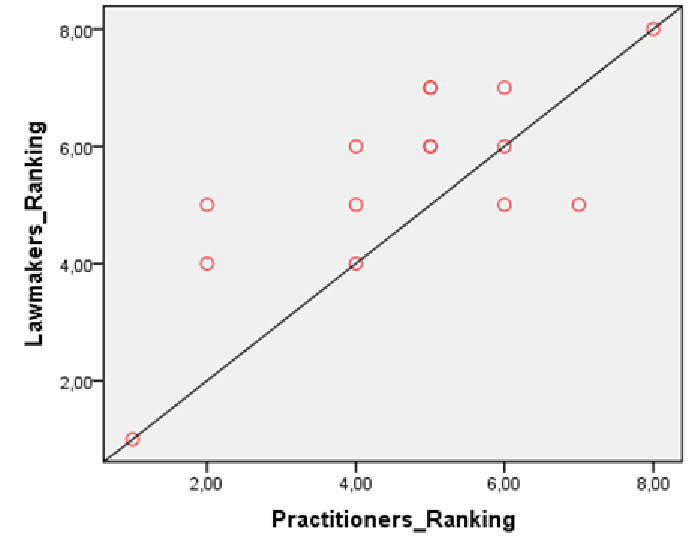
\includegraphics[width=0.4\textwidth]{Figures/Chall_ranking.drawio.pdf} 
%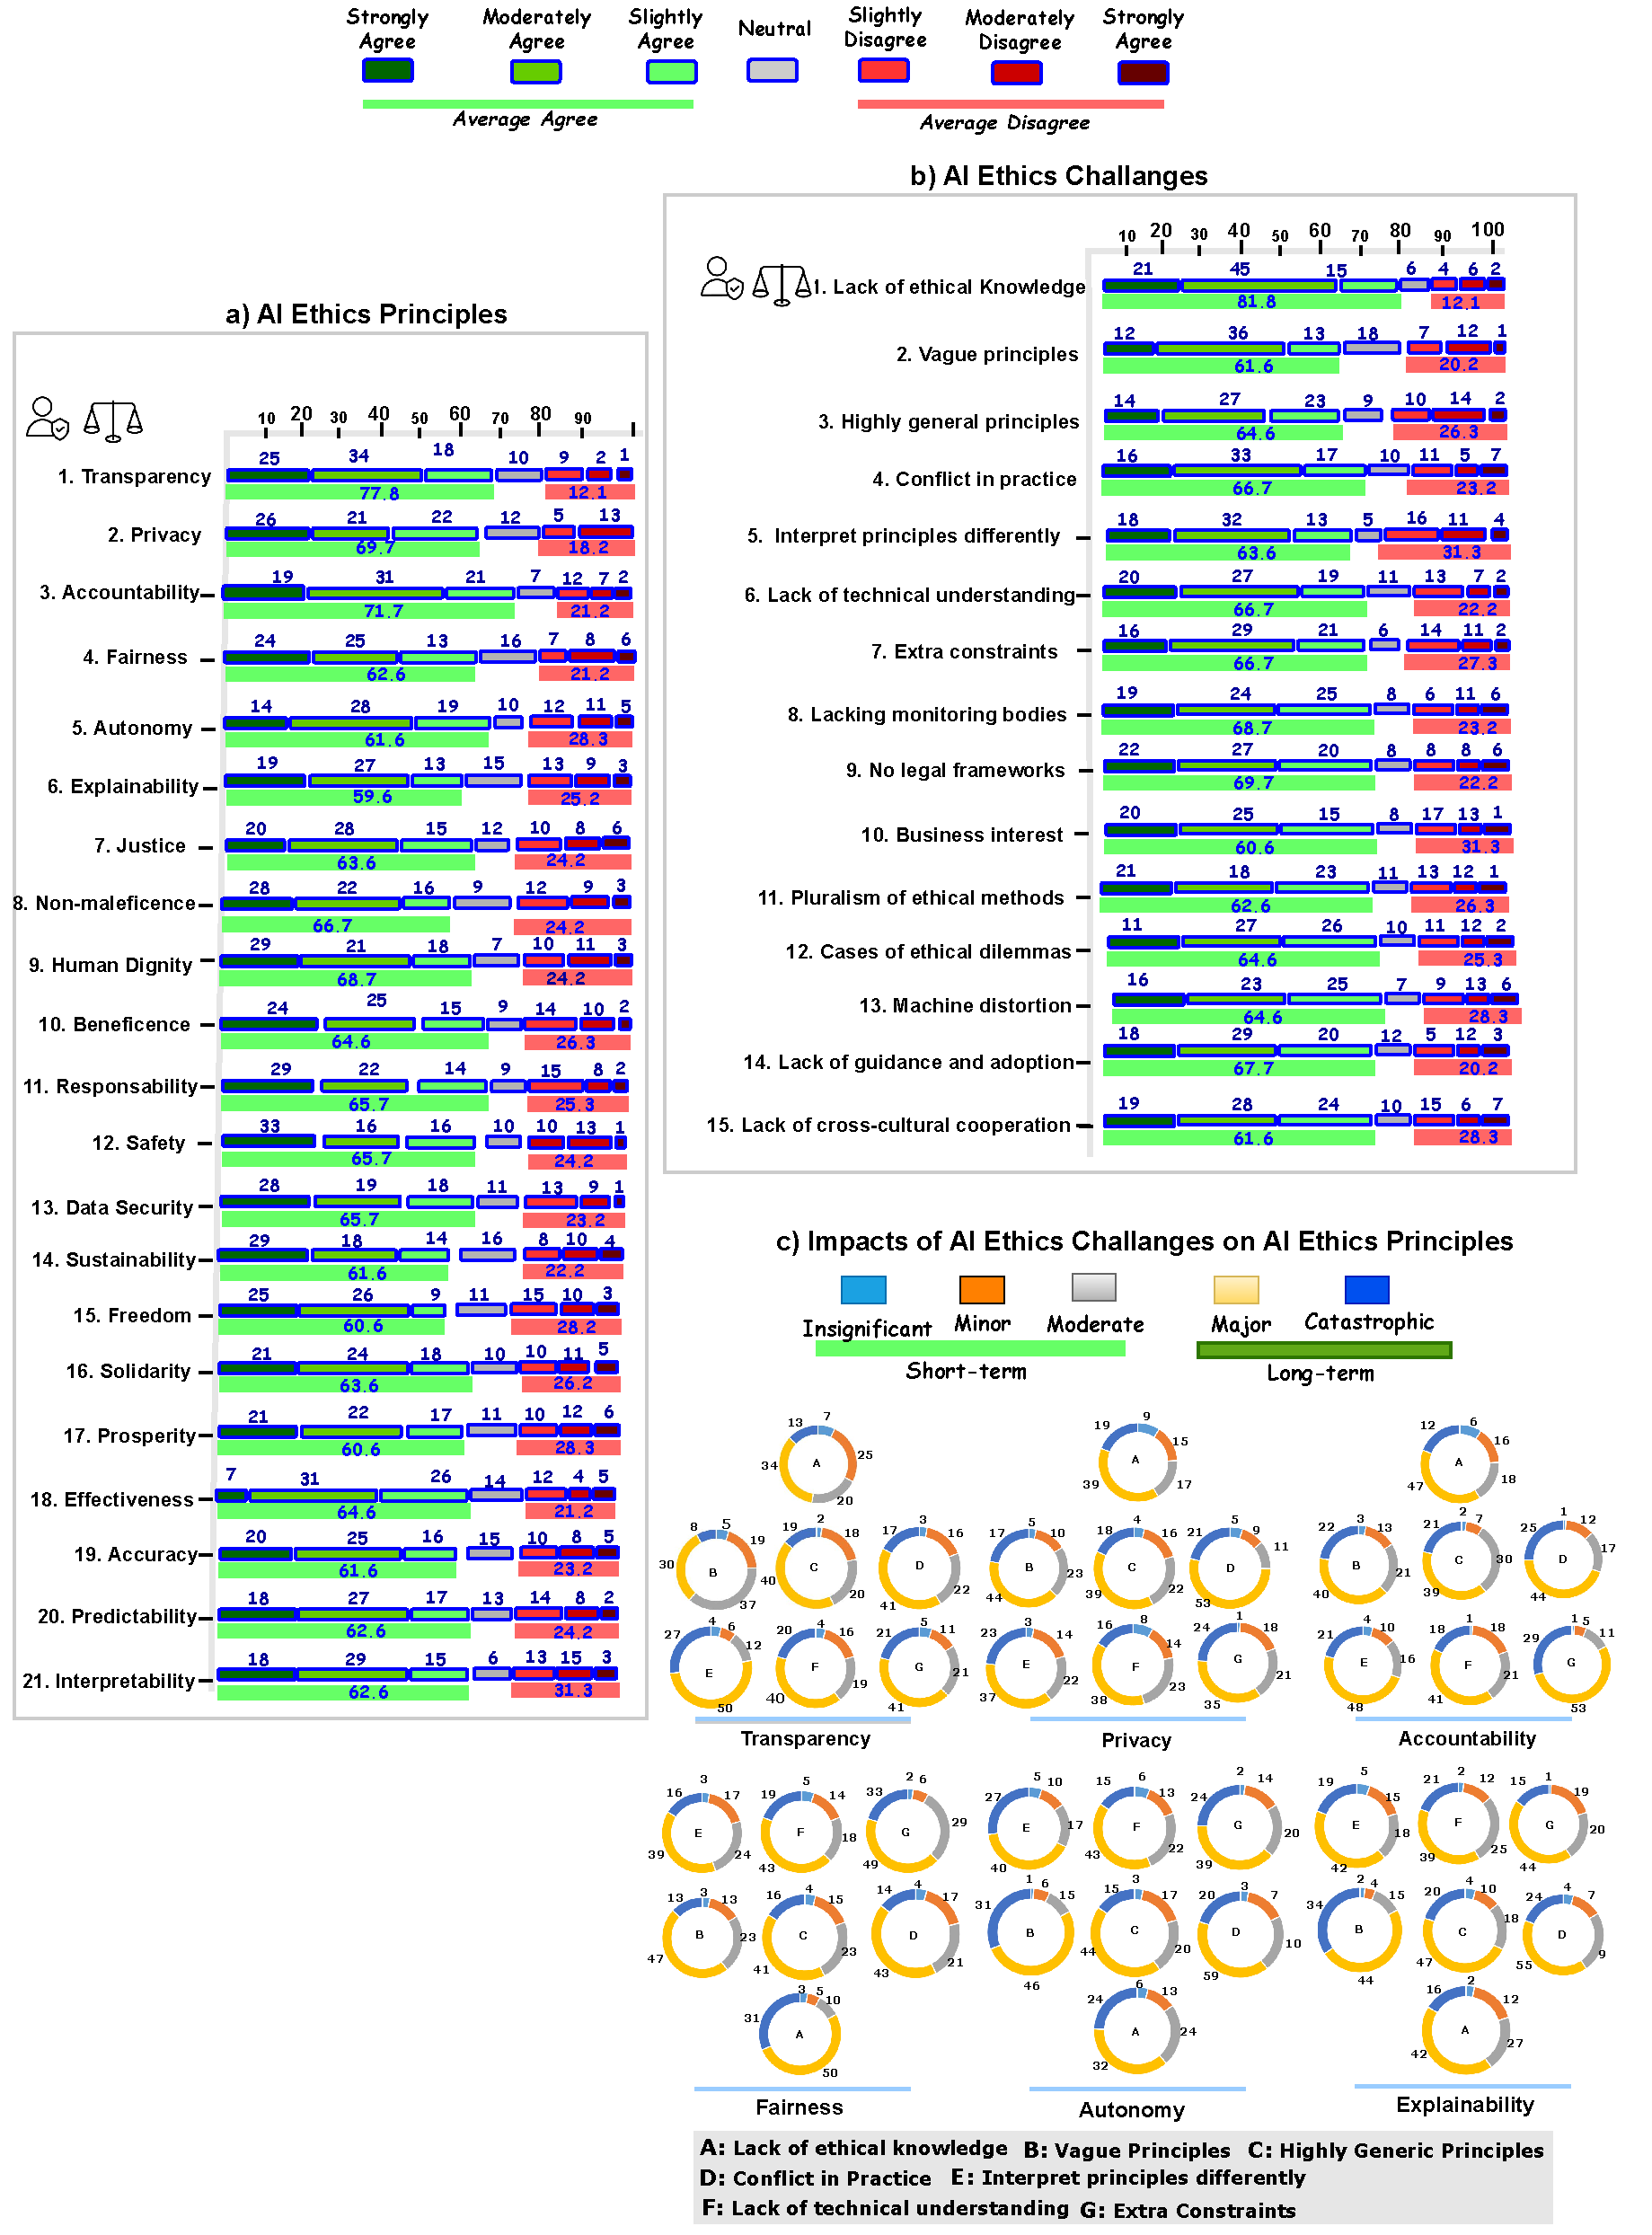
\includegraphics[width=\textwidth]{Figures/SurveyFindings.pdf}
 	\caption{Scatter plot of ranks for AI ethics challenges}
	\label{Fig:Scatter-Ranks-challenges}
\end{figure}

We also applied the independent t-test (see Table \ref{tab:ttest-challenges}, Table \ref{tab:group-stat-challenges}) to assess the mean differences between both types of the population with respect to AI ethics challenges. The calculated significance value of Levene's Test is (p$=$0.051$>$0.05); therefore, we assume the variances equally (see Table \ref{tab:ttest-challenges}). The t-test results, assuming equal variances (t$=$1.291, p$=$0.207$>$0.05), show that practitioners and lawmakers consider the signaficance of identified challenges equally. We could suppose that practitioners and lawmakers are equally aware of the reported challenges and understand their importance. The group statistics for both variables are provided in Table \ref{tab:group-stat-challenges}.
 
% Please add the following required packages to your document preamble:
% \usepackage{multirow}
% \usepackage{graphicx}
\begin{table*}[]
\centering
\caption{Practitioners and lawmakers perceptions co-relation for AI ethics challenges}
\label{tab:corr_challenges}
% \resizebox{\textwidth}{!}{%
\begin{tabular}{|lllll|}
\hline
\multicolumn{5}{|l|}{Correlations} \\ \hline
\multicolumn{3}{|l|}{} & \multicolumn{1}{l|}{Lawmakers\_Ranking} & Practitioners\_Ranking \\ \hline
\multicolumn{1}{|l|}{\multirow{6}{*}{Spearman's rho}} & \multicolumn{1}{l|}{\multirow{3}{*}{Lawmakers\_Ranking}} & \multicolumn{1}{l|}{Correlation Coefficient} & \multicolumn{1}{l|}{1.000} & 0.628* \\ \cline{3-5} 
\multicolumn{1}{|l|}{} & \multicolumn{1}{l|}{} & \multicolumn{1}{l|}{Sig. (2-tailed)} & \multicolumn{1}{l|}{.} & 0.012 \\ \cline{3-5} 
\multicolumn{1}{|l|}{} & \multicolumn{1}{l|}{} & \multicolumn{1}{l|}{N} & \multicolumn{1}{l|}{15} & 15 \\ \cline{2-5} 
\multicolumn{1}{|l|}{} & \multicolumn{1}{l|}{\multirow{3}{*}{Practitioners\_Ranking}} & \multicolumn{1}{l|}{Correlation Coefficient} & \multicolumn{1}{l|}{0.628*} & 1.000 \\ \cline{3-5} 
\multicolumn{1}{|l|}{} & \multicolumn{1}{l|}{} & \multicolumn{1}{l|}{Sig. (2-tailed)} & \multicolumn{1}{l|}{0.012} & . \\ \cline{3-5} 
\multicolumn{1}{|l|}{} & \multicolumn{1}{l|}{} & \multicolumn{1}{l|}{N} & \multicolumn{1}{l|}{15} & 15 \\ \hline
\multicolumn{5}{|l|}{*.   Correlation is significant at the 0.05 level (2-tailed).} \\ \hline
\end{tabular}%
% }
\end{table*}

% Please add the following required packages to your document preamble:
% \usepackage{multirow}
% \usepackage{graphicx}
\begin{table*}[]
\centering
\caption{Independent samples t-test of AI ethics challenges}
\label{tab:ttest-challenges}
\resizebox{\textwidth}{!}{%
\begin{tabular}{|ll|ll|lllllll|}
\hline
\multicolumn{2}{|l|}{\multirow{3}{*}{}} & \multicolumn{2}{l|}{\begin{tabular}[c]{@{}l@{}}Levene's Test   for  \\    \\ Equality of   Variances\end{tabular}} & \multicolumn{7}{l|}{t-test for   Equality of Means} \\ \cline{3-11} 
\multicolumn{2}{|l|}{} & \multicolumn{1}{l|}{\multirow{2}{*}{F}} & \multirow{2}{*}{Sig.} & \multicolumn{1}{l|}{\multirow{2}{*}{t}} & \multicolumn{1}{l|}{\multirow{2}{*}{df}} & \multicolumn{1}{l|}{\multirow{2}{*}{\begin{tabular}[c]{@{}l@{}}Sig. (2-   \\    \\ tailed)\end{tabular}}} & \multicolumn{1}{l|}{\multirow{2}{*}{\begin{tabular}[c]{@{}l@{}}Mean  \\    \\ Difference\end{tabular}}} & \multicolumn{1}{l|}{\multirow{2}{*}{Std. Error  Difference}} & \multicolumn{2}{l|}{\begin{tabular}[c]{@{}l@{}}95\% Confidence  \\    \\ Interval of the    \\    \\ Difference\end{tabular}} \\ \cline{10-11} 
\multicolumn{2}{|l|}{} & \multicolumn{1}{l|}{} &  & \multicolumn{1}{l|}{} & \multicolumn{1}{l|}{} & \multicolumn{1}{l|}{} & \multicolumn{1}{l|}{} & \multicolumn{1}{l|}{} & \multicolumn{1}{l|}{Lower} & Upper \\ \hline
\multicolumn{1}{|l|}{\multirow{2}{*}{Rank}} & Equal variances  assumed & \multicolumn{1}{l|}{.519} & .477 & \multicolumn{1}{l|}{1.291} & \multicolumn{1}{l|}{28} & \multicolumn{1}{l|}{.207} & \multicolumn{1}{l|}{.86667} & \multicolumn{1}{l|}{.67141} & \multicolumn{1}{l|}{-.50866} & 2.24199 \\ \cline{2-11} 
\multicolumn{1}{|l|}{} & Equal variances  not assumed & \multicolumn{1}{l|}{} &  & \multicolumn{1}{l|}{1.291} & \multicolumn{1}{l|}{27.145} & \multicolumn{1}{l|}{.208} & \multicolumn{1}{l|}{.86667} & \multicolumn{1}{l|}{.67141} & \multicolumn{1}{l|}{-.51061} & 2.24395 \\ \hline
\end{tabular}%
}
\end{table*}

% Please add the following required packages to your document preamble:
% \usepackage{multirow}
% \usepackage{graphicx}
\begin{table*}[]
\centering
\caption{AI ethic challenges group statistics}
\label{tab:group-stat-challenges}
% \resizebox{0.6\textwidth}{!}{%
\begin{tabular}{|l|l|l|l|l|l|}
\hline
 & group & N & Mean & Std. Deviation & Std. Error Mean \\ \hline
\multirow{2}{*}{Rank} & lawmakers & 15 & 5.1333 & 1.99523 & .51517 \\ \cline{2-6} 
 & practitioners & 15 & 4.2667 & 1.66762 & .43058 \\ \hline
\end{tabular}%
% }
\end{table*}
Overall, we believe that practitioners and lawmakers are on the same page in considering AI ethics principles and challenges. 
However, for AI ethics challenges, the perceptions of practitioners and lawmakers are slightly different. 
We noticed that various AI ethics principles and guidelines are released in private and public sectors, which are very abstract, and incoherent for various stakeholders to implement \cite{munn2022uselessness}. The challenges of interpreting these vague principles are different with respect to the targeted group of stakeholders e.g., industrial and legislation perspectives \cite{munn2022uselessness}. In conclusion, there is a gap between high-minded principles and industrial practices, which needs alternative approaches based on mutual industrial and legislation consensus.

